\section{Results}\label{sec:results}
For our experiments, we used a Red Hat 8 server with a Intel Xeon Gold 6242
CPU. Since \shortname{} is written in Rust, it mostly uses the built-in
functionality of the egg library. The egg e-graph runner was ran in a
time-limited configuration, meaning there was no limit in the size of the
e-graph or number of rewrite iterations. The specific time limit for e-graph
construction was 10 minutes. In most cases, the test circuit saturated the
e-graph well before this time limit \todo{Berk, do we have avg eqsat time?}.
\shortname{} was evaluated against circuits from three benchmark suites:
EPFL~\cite{epflbench}, ISCAS'85~\cite{iscasbench}, and
LGSynth'91~\cite{lgsynthbench}. However, we also included an ALU and pipelined
multiplication module to test how our compiler behaves with increasing levels
of bit-parallelism and pipeline stages. Finally, we measure how our mapping
optimizations influence CLB usage and timing closure.

\subsection{Benchmarking}\label{sec:results:benchmark}
\begin{table}
    \centering
    \csvautobooktabular{data/results.csv}
    \caption{Results of 30 improved benchmarks from ISCAS'85~\cite{iscasbench}, LGSynth'91~\cite{lgsynthbench}, and EPFL~\cite{epflbench}}\label{tab:results}
\end{table}

We used an compilation of 96 combinational benchmarks from three academic
sources to test LUT packing ability. Among the combinational benchmarks we
tested, \shortname{} was able to reduce the LUT count \fmetric{} of the time.
On average, \shortname{} packed the netlists to \metric{}. The results in
Table~\ref{tab:results} list the all the reduced LUT counts, sorted by
approximate design size. AMD, formerly Xilinx, Vivado 2022~\cite{vivado} was
used as the baseline synthesis tool. For the E-Pack flow, Yosys~\cite{yosys} is
used to generate the initial mapped circuit. \todo{Do we have anything to say
    about term1, int2float, i5, c6288, adder, and sqaure?}

One result that is not illustrated in the table is the apparent importance of
the initial structure inputted to E-Pack. We have not eliminated all sources of
structural bias, and hence our superoptimization tool still occasionally gets
stuck at a local minimum. Future work will investigate which qualities make a
RTL synthesis engine work well with our tool versus ones that do not. For
example, E-Pack optimized Yosys 0.33 netlists better than ones provided by
Yosys 0.47. Likewise, future work will experiment with rewrite procedures than
can break out of these local minimums on their own.

\subsection{Marginal Improvement and Time Cost}\label{sec:results:margin}
\begin{figure}
    \begin{subfigure}{0.47\textwidth}
        \centering
        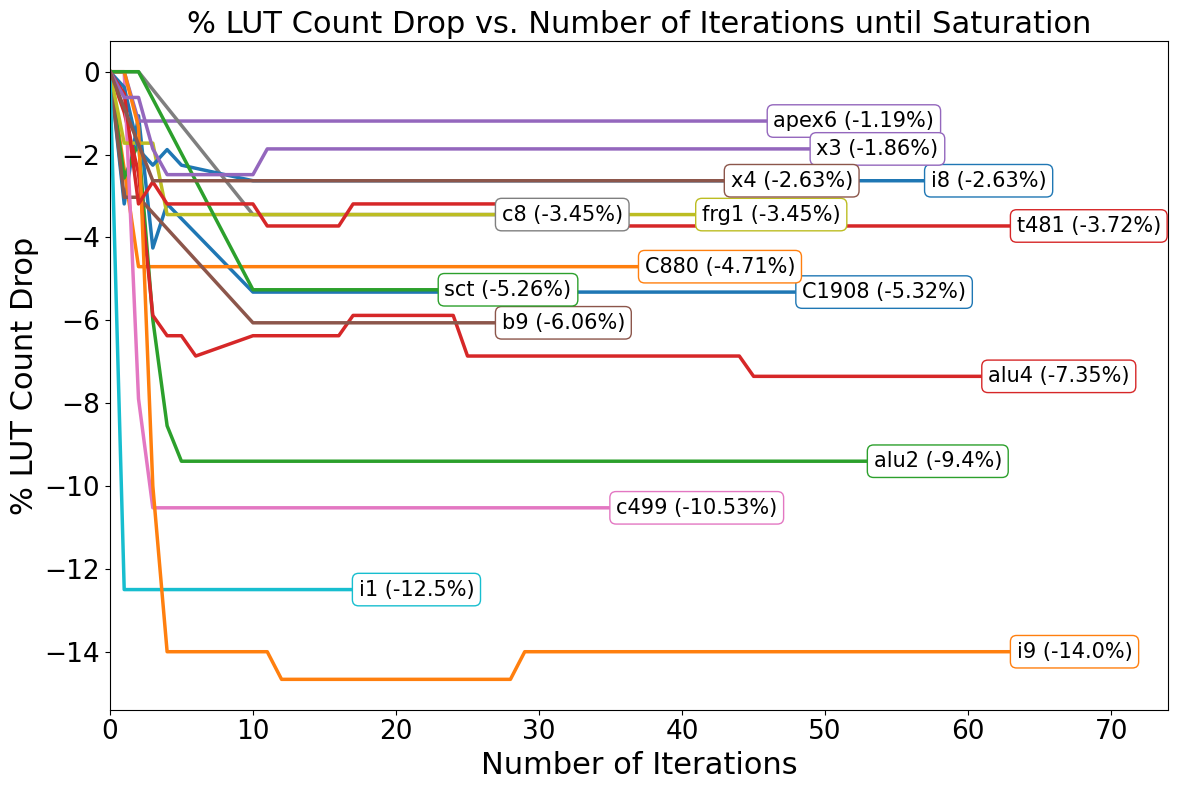
\includegraphics[width=\textwidth]{img/improvement.png}
        \caption{Marginal improvement versus iteration count. The labels mark the equality saturation point.}\label{fig:marginal:improvement}
        \Description[]{}
    \end{subfigure}
    \hfill\vspace{4mm}
    \begin{subfigure}{0.47\textwidth}
        \centering
        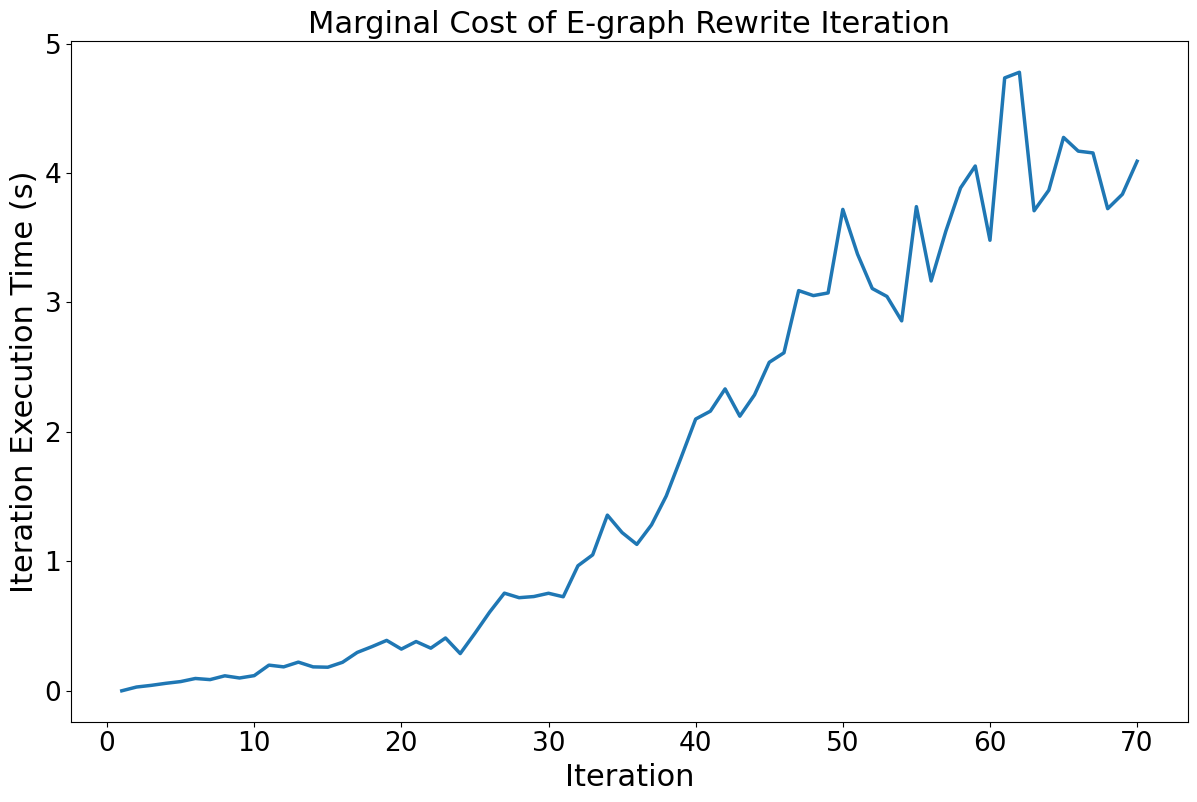
\includegraphics[width=\textwidth]{img/runtime_derivative.png}
        \caption{Marginal increase in runtime versus iteration count. Later iterations consume more time as the graph is larger.}\label{fig:marginal:runtime}
        \Description[]{}
    \end{subfigure}
    \caption{Comparison between gains in QoR against increasing execution time with graph size. Running a netlist to equality saturation requires more rewrite iterations, and hence a larger e-graph.}\label{fig:marginal}
    \Description[]{}
\end{figure}
\todo{explain graph showing improvement with iter count}

\subsection{Case Study: Pipelined Designs}\label{sec:results:retiming}
\begin{table*}[t]
    \centering
    \csvautobooktabular{data/mult.csv}
    \caption{LUT and flip-flop counts are report post-synthesis, but before placement and routing. CLB counts are reported after placement and routing.}\label{tab:multiply}
\end{table*}

Hardware designs with feed forward pipelines provide interesting opportunities
to apply register retiming and find a higher-level of area optimization. When
closing timing on FPGA designs, the critical path is often dominated by the
effects of routing congestion, moreso than ASIC design. Hence, reducing the
cell count and circuit depth along the delay path is a valid optimization
strategy for FPGA design. As a caveat, it is important to note that other work
has also observed the opposite trend~\cite{academicfpga}: decreasing depth too
much can strain the router. In any case, E-Pack can be utilized to reduce total
CLB usage. To elaborate, every CLB in the Ultrascale+ architecture contains 1
slice, which itself contains 8 LUTs and 16 flip-flops~\cite{ug574}.
Intuitively, a design that maps to CLBs efficiently will contain more
flip-flops than LUTs due to this 2:1 ratio. To test this hypothesis,
Table~\ref{tab:multiply} shows the results of a pipelined multiplier with a
varying number of pipeline stages processed with E-Pack.

While the total drop is CLB usage is desirable, the area gains as a percentage
are modest due to the suboptimality of greedy e-graph extraction. Register
retiming rewrites, when enabled, vastly increase the design space. More
importantly, register retiming changes the topology of the stateful
elements---i.e. the flip-flops. As a consequence, greedy extraction cannot take
into account the fanout of flip-flops. It chooses a poor design point with less
register fanout and a greater total number of registers. The few regressions
observed in mapping combinational logic (Fig.~\ref{fig:marginal:improvement})
become more frequent and exacerbated in sequential logic. While these results
\textit{do} demonstrate that optimizing for CLB count over raw cell count is a
feasible strategy, a different extraction method will be needed in future work.

\subsection{Case Study: Bit-Parallel Designs}\label{sec:results:scalability}
\begin{table}
    \centering
    \csvautobooktabular{data/alu.csv}
    \caption{Synthesis results of $n$-bit ALU}\label{tab:alu}
\end{table}
\todo{explain increasing ALU bit parallelism}
